\section{Shadow DOM}\label{shadow-dom}

\begin{itemize}
\item
  TODO:
\item
  Ausformulieren:
\item
  Complete
\end{itemize}

\subsection{Einführung}\label{einfuxfchrung}

\begin{itemize}
\tightlist
\item
  Der Shadow DOM ist ein Sub-DOM unterhalb einem HTML Element, der es
  ermöglicht, HTML und CSS in sich zu kapseln und zu verstecken
\item
  Wird Shadow DOM wird bereits in HTML5 standardmäßig eingesetzt, z.b.
  in dem \texttt{\textless{}video\textgreater{}} Tag. Beim Inspizieren
  wird deutlich, dass das \texttt{\textless{}video\textgreater{}} Tag
  einen Shadow DOM beinhaltet, welcher die Steuerelemente des Videos
  erzeugt
\item
  Ebenso sind die verschiedenen \texttt{\textless{}input\textgreater{}}
  Elemente, wie z.B. das
  \texttt{\textless{}input\ type="password"\textgreater{}} mit einem
  Shadow-DOM ausgestattet:
\end{itemize}

\begin{figure}[htbp]
\centering
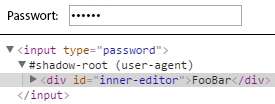
\includegraphics{images/2-shadow-dom-input-type-password.jpg}
\caption{Bild: input type=`password' Element}
\end{figure}

\begin{itemize}
\tightlist
\item
  Der Shadow DOM liegt dabei parallel zu dem DOM Knoten des
  beinhaltenden Elementes (Siehe Bild). Ein Knoten im Document tree
  (links) wird als Shadow DOM beihaltendes Element (shadow host)
  markiert. Die gestrichelte Linie zeigt die Referenz zu der
  entsprechenden Shadow DOM Wurzel, dem ``shadow root''. Die Referenz
  geht dabei durch die sogenannte ``Shadow Boundary'', welche es
  ermöglicht, den Shadow DOM, und alles was dieser beinhaltet, zu
  kapseln
\item
  Die Kapselung des Shadow DOM mittels der Shadow Boundary verhindert,
  dass CSS oder JavaScript in den Shadow DOM hinein oder hinaus kommen
\end{itemize}

\begin{figure}[htbp]
\centering
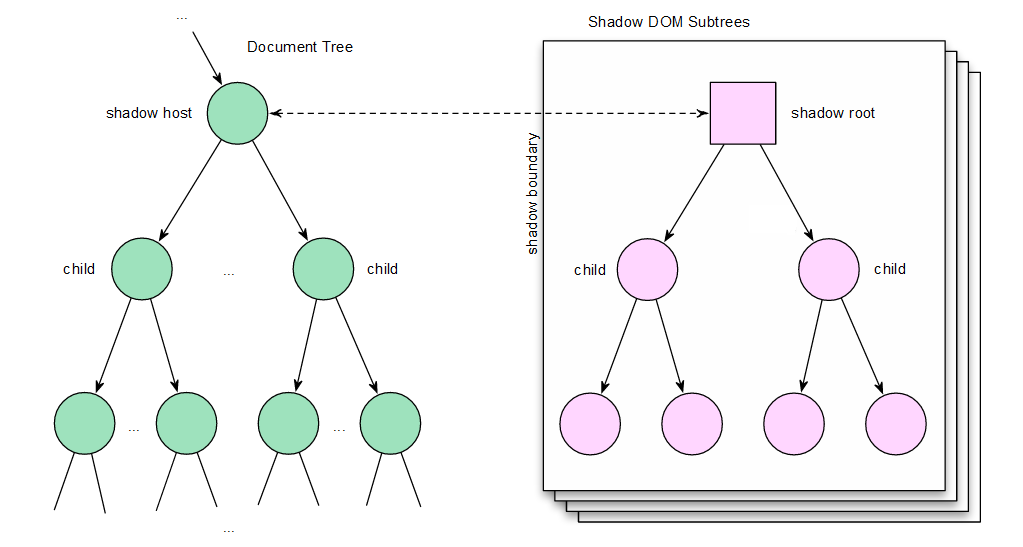
\includegraphics{images/2-shadow-dom-shadow-boundary.png}
\caption{Bild: Shadow DOM und Shadow Boundary nach W3C}
\end{figure}

\begin{itemize}
\tightlist
\item
  Ein Element kann auch mehrere Shadow DOM Wurzeln referenzieren,
  allerdings wird nur die zuletzt hinzugefügte gerendert, der Browser
  benutzt beim Rendern einen LIFO Stack
\item
  Der zuletzt hinzugefügte Shadow Tree wird ``youngest tree'' genannt,
  der jeweils zuvor hinzugefügte Shadow Tree wird ``older tree'' genannt
\end{itemize}

{[}Colin Ihrig 2012{]}, {[}Peter Kröner 2014{]}

\subsection{Content projecting}\label{content-projecting}

\begin{itemize}
\tightlist
\item
  Neben dem vom Shadow DOM vorgegebenen HTML Markup, können auch Inhalte
  aus dem Shadow DOM in den Light DOM, den DOM des Dokumentes,
  projiziert werden.
\item
  Der Shadow DOM ermöglicht somit die Möglichkeit gekapseltes HTML im
  Shadow DOM, sowie dynamische Inhalte im Light DOM anzuzeigen
\item
  Diese Projektion der Inhalte in den Light DOM erfolgt mittels
  ``Insertion Points'', wobei zwischen zwei Arten von ``Insertion
  Points'' unterschieden wird:
\end{itemize}

\subsubsection{Insertion Points}\label{insertion-points}

\begin{itemize}
\tightlist
\item
  Um das zu präsentierende HTML von dem notwendigen zu trennen, wird ein
  \texttt{\textless{}template\textgreater{}} Tag benutzt. Dieses
  beinhaltet alles Markup, das im Shadow DOM stehen und nicht nach außen
  sichtbar oder manipuliert werden soll
\item
  Das \texttt{\textless{}template\textgreater{}} Tag kann nun ein
  \texttt{\textless{}content\textgreater{}} Tag beinhalten, welches die
  Inhalte von außen in den Light DOM hineinprojiziert. Der Light DOM ist
  der DOM des HTML Dokumentes
\end{itemize}

\begin{Shaded}
\begin{Highlighting}[]
\KeywordTok{<div}\OtherTok{ id=}\StringTok{"shadow"}\KeywordTok{>}\NormalTok{Content}\KeywordTok{</div>}
\KeywordTok{<template}\OtherTok{ id=}\StringTok{"myTemplate"}\KeywordTok{>}
  \KeywordTok{<div}\OtherTok{ class}\ErrorTok{"hiddenWrapper"}\KeywordTok{>}
    \KeywordTok{<content></content>}
  \KeywordTok{</div>}
\KeywordTok{</template>}
\end{Highlighting}
\end{Shaded}

\begin{Shaded}
\begin{Highlighting}[]
\OperatorTok{<}\NormalTok{script}\OperatorTok{>}
\KeywordTok{var} \NormalTok{shadow }\OperatorTok{=} \VariableTok{document}\NormalTok{.}\AttributeTok{querySelector}\NormalTok{(}\StringTok{'#shadow'}\NormalTok{).}\AttributeTok{createShadowRoot}\NormalTok{()}\OperatorTok{;}
\KeywordTok{var} \NormalTok{template }\OperatorTok{=} \VariableTok{document}\NormalTok{.}\AttributeTok{querySelector}\NormalTok{(}\StringTok{'#myTemplate'}\NormalTok{)}\OperatorTok{;}
\KeywordTok{var} \NormalTok{clone }\OperatorTok{=} \VariableTok{document}\NormalTok{.}\AttributeTok{importNode}\NormalTok{(}\VariableTok{template}\NormalTok{.}\AttributeTok{content}\OperatorTok{,} \KeywordTok{true}\NormalTok{)}\OperatorTok{;}
\VariableTok{shadow}\NormalTok{.}\AttributeTok{appendChild}\NormalTok{(clone)}\OperatorTok{;}
\OperatorTok{<}\SpecialStringTok{/script>}
\end{Highlighting}
\end{Shaded}

\begin{itemize}
\tightlist
\item
  Gerendert wird dabei nur ``Content'' des divs mit der id ``shadow'',
  der Wrapper um das \texttt{\textless{}content\textgreater{}} Tag wird
  nicht gerendert, da dieser im Shadow DOM steht
\item
  Somit wurde eine Trennung des Inhalts und der Darstellung erreicht,
  der Inhalt steht im Dokument, die Darstellung erfolgt im Shadow DOM
\item
  Nodes die aus dem Host ein den Shadow Tree projiziert werden heißen
  ``distributed nodes''
\item
  Es können auch nur bestimmte Elemente in den Light DOM projiziert
  werden, ermöglicht wird dies mit dem Attribut \texttt{select} des
  \texttt{content} Tags. Dabei können Elemente, sowie CSS Selektoren
  verwendet werden
\item
  HTML Elemente, die via \texttt{\textless{}content\textgreater{}} und
  \texttt{\textless{}content\ select="element"\textgreater{}} in den
  Light DOM projiziert werden, können somit auch von außen gestyled
  werden (zusätzlich auch via ::content - siehe ``Styling mit CSS'')
\end{itemize}

{[}Eric Bidelman 2013{]}

\subsubsection{Shadow Insertion Points}\label{shadow-insertion-points}

\begin{itemize}
\tightlist
\item
  \texttt{\textless{}shadow\textgreater{}} Insertion Points sind, ebenso
  wie \texttt{\textless{}content\textgreater{}} Insertion Points,
  Platzhalter, doch statt einem Platzhalter für den Inhalt eines Hosts,
  sind sie Platzhalter für Shadow Trees
\item
  Wenn nun mehrere Shadow Trees gerendert werden sollen, muss im zuletzt
  hinzugefügten Shadow Tree (younger tree) ein
  \texttt{\textless{}shadow\textgreater{}} Tag stehen, dieser rendert
  den zuvor hinzugefügten Shadow Tree (older tree), somit wird eine
  Shadow DOM Schachtelung ermöglicht
\end{itemize}

{[}Eric Bidelman 2014{]}

\subsection{Styling mit CSS}\label{styling-mit-css}

\begin{itemize}
\item
  Shadow Boundary: Styles gehen nicht aus Shadow Dom raus, und keine
  rein. -\textgreater{} Style Kapselung ``out of the box''!
\item
  Styling des host-Elements mit :host \emph{selector} -\textgreater{}
  Allerdings überschreiben die inneren Styles nicht die Äußeren! (Siehe
  snippets/shadow-dom/\#styling) -\textgreater{} Wichtig bei ``Reacting
  to user states''
\item
  Styling des Hosts in Abhängigkeit des Kontextes mit :host-context
  (https://drafts.csswg.org/css-scoping/\#selectordef-host-context) z.B.
  :host-context(.wrapper)
\item
  Styling des Shadow DOM von außerhalb
\item
  ::shadow

  \begin{itemize}
  \tightlist
  \item
    z.b.: my-element::shadow .content \{\} spricht .content elemente IN
    einem Shadow DOM an
  \item
    Styled alle elemente in DIESEM Shadow DOM
  \end{itemize}
\item
  \begin{quote}
  \begin{quote}
  \begin{quote}
  (ehem. /deep/)
  (https://drafts.csswg.org/css-scoping-1/\#deep-combinator)
  \end{quote}
  \end{quote}
  \end{quote}

  \begin{itemize}
  \tightlist
  \item
    z.b.: my-element \textgreater{}\textgreater{}\textgreater{}
    .different spricht ALLE .different Elemente in my-element an, egal
    wieviele Shadow DOMS noch darunter geschachtelt sind
  \item
    So können z.B. ``Style-hooks'' erzeugt werden, die es Entwicklern
    ermöglicht eigene Styles auf ein Component zu binden some-element
    \textgreater{}\textgreater{}\textgreater{} .custom-theme \{ \ldots{}
    \}
  \end{itemize}
\item
  ::slotted (ehem. ::content)
  (http://www.html5rocks.com/en/tutorials/webcomponents/shadowdom-201/\#toc-distributed)

  \begin{itemize}
  \tightlist
  \item
    Elemente, die in ein \texttt{\textless{}content\textgreater{}}
    projiziert werden, können auch von innen gestyled werden, z.B. (in
    einer Komponente):
  \end{itemize}

  \texttt{CSS\ \ \ ::slotted\ p\ \{\ \ \ \ \ color:\ red;\ \ \ \}}

  \begin{itemize}
  \tightlist
  \item
    Spricht alle \texttt{\textless{}p\textgreater{}} in einem
    \texttt{\textless{}content\textgreater{}} Tag an, die in dem Light
    DOM projiziert werden.
  \end{itemize}
\item
  CCS Variablen (http://dev.w3.org/csswg/css-variables/)

  \begin{itemize}
  \tightlist
  \item
    Eine Komponente hält im Inneren Variablen für das Aussehen, somit
    wir das Styling nach außen gegeben z.B.:
  \end{itemize}

  \texttt{CSS\ \ \ my-button\ \{\ \ \ \ \ color:\ var(-\/-button-theme-color,\ red);\ \ \#(red\ wäre\ default)\ \ \ \ \ font-family:\ var(-\/-button-theme-font);\ \ \ \}}
  Der Entwickler kann nun von außen die Variablen instanzieren mit

  \texttt{CSS\ \ \ \#host\ \{\ \ \ \ \ -\/-button-theme-color:\ red;\ \ \ \ \ -\/-button-theme-font:\ \ Arial;\ \ \ \}}
\item
  Mit ::shadow und \textgreater{}\textgreater{}\textgreater{} können
  native Elemente, die einen Shadow DOM benutzen, gestyled werden, wie
  z.B. \texttt{\textless{}video\textgreater{}} oder
  \texttt{\textless{}input\textgreater{}} Elemente
\item
  Jedoch sprengt das das Prinzip der Kapselung, das man mit Web
  Components versucht zu gewinnen, jedoch sollten Web Entwickler
  natürlich dennoch die Möglichkeit haben, fremde Components zu stylen,
  wenn sie wissen was sie machen.
\item
  Alles wird durch Polyfills abgedeckt
\end{itemize}

{[}Eric Bidelman 2014{]}, {[}Rob Dodson 2014{]}

\subsection{Beispiel eines Shadow DOMs mit Template und CSS
Styles}\label{beispiel-eines-shadow-doms-mit-template-und-css-styles}

\begin{itemize}
\tightlist
\item
  Soll nun ein einfacher Shadow DOM mit gekapseltem CSS und JavaScript
  erzeugt werden, könnte dies folgendermaßen erfolgen:
\end{itemize}

\begin{Shaded}
\begin{Highlighting}[]
\KeywordTok{<style>}
  \FloatTok{.styled} \KeywordTok{\{}
    \KeywordTok{color:} \DataTypeTok{green}\KeywordTok{;}
  \KeywordTok{\}}
  \FloatTok{.content} \KeywordTok{\{}
    \KeywordTok{background-color:} \NormalTok{khaki}\KeywordTok{;}
  \KeywordTok{\}}
\KeywordTok{</style>}

\KeywordTok{<div}\OtherTok{ id=}\StringTok{"hello"}\KeywordTok{>}
  \KeywordTok{<div>}\NormalTok{Hello}\KeywordTok{</div>}
  \KeywordTok{<div}\OtherTok{ class=}\StringTok{"styled"}\KeywordTok{>}\NormalTok{Styled}\KeywordTok{</div>}
  \KeywordTok{<p}\OtherTok{ class=}\StringTok{"hidden"}\KeywordTok{>}\NormalTok{Hidden Content}\KeywordTok{</p>}
\KeywordTok{</div>}
\KeywordTok{<template}\OtherTok{ id=}\StringTok{"myTemplate"}\KeywordTok{>}
  \KeywordTok{<style>}
    \FloatTok{.wrapper} \KeywordTok{\{}
      \KeywordTok{border:} \DataTypeTok{2px} \DataTypeTok{solid} \DataTypeTok{black}\KeywordTok{;}
      \KeywordTok{width:} \DataTypeTok{120px}\KeywordTok{;}
    \KeywordTok{\}}
    \FloatTok{.content} \KeywordTok{\{}
      \KeywordTok{color:} \DataTypeTok{red}\KeywordTok{;}
    \KeywordTok{\}}
  \KeywordTok{</style>}

  \KeywordTok{<div}\OtherTok{ class=}\StringTok{"wrapper"}\KeywordTok{>}
    \NormalTok{Shadow DOM}
    \KeywordTok{<div}\OtherTok{ class=}\StringTok{"content"}\KeywordTok{>}
      \KeywordTok{<content}\OtherTok{ select=}\StringTok{"div"}\KeywordTok{></content>}
    \KeywordTok{</div>}
  \KeywordTok{</div>}
\KeywordTok{</template>}

\KeywordTok{<script>}
  \KeywordTok{var} \NormalTok{root }\OperatorTok{=} \VariableTok{document}\NormalTok{.}\AttributeTok{querySelector}\NormalTok{(}\StringTok{'#hello'}\NormalTok{).}\AttributeTok{createShadowRoot}\NormalTok{()}\OperatorTok{;}
  \KeywordTok{var} \NormalTok{template }\OperatorTok{=} \VariableTok{document}\NormalTok{.}\AttributeTok{querySelector}\NormalTok{(}\StringTok{'#myTemplate'}\NormalTok{)}\OperatorTok{;}
  \KeywordTok{var} \NormalTok{clone }\OperatorTok{=} \VariableTok{document}\NormalTok{.}\AttributeTok{importNode}\NormalTok{(}\VariableTok{template}\NormalTok{.}\AttributeTok{content}\OperatorTok{,} \KeywordTok{true}\NormalTok{)}\OperatorTok{;}
  \VariableTok{root}\NormalTok{.}\AttributeTok{appendChild}\NormalTok{(clone)}\OperatorTok{;}
\OperatorTok{<}\SpecialStringTok{/script>}
\end{Highlighting}
\end{Shaded}

\begin{itemize}
\tightlist
\item
  Das Beispiel oben wird vom Browser wie folgt gerendert:
\end{itemize}

\begin{figure}[htbp]
\centering
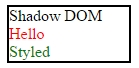
\includegraphics{images/2-shadow-dom-beispiel.jpg}
\caption{Bild: Shadow DOM Beispiel}
\end{figure}

\begin{itemize}
\tightlist
\item
  Hier sind einige Dinge anzumerken:
\item
  Es werde per select im \texttt{\textless{}content\textgreater{}} nur
  die divs aus dem Shadow Root mit der ID ``hello'' gerendert, der
  Paragrapg mit der ID ``hidden wird nicht gerendert
\item
  Die CSS Regel \texttt{.content\ \{\ background-color:\ khaki;\ \}} des
  HTML Dokumentes greift nicht durch die Shadow Boundary
\item
  Die CSS Regel \texttt{.styled\ \{\ color:\ green;\ \}} greift, da der
  div mit der Klasse ``.styled'' in den Light DOM projiziert wird
\item
  Innerhalb des Templates können CSS Regeln für die beinhaltenden
  Elemente definiert werden
\end{itemize}

\subsection{Browserunterstützung}\label{browserunterstuxfctzung}

\begin{itemize}
\tightlist
\item
  Noch nicht standardtisiert, sind noch ein Working Draft
  (http://www.w3.org/TR/shadow-dom/)
\item
  Deshalb bisher auch nur in Chrome und Opera unterstützt
\end{itemize}

\begin{figure}[htbp]
\centering
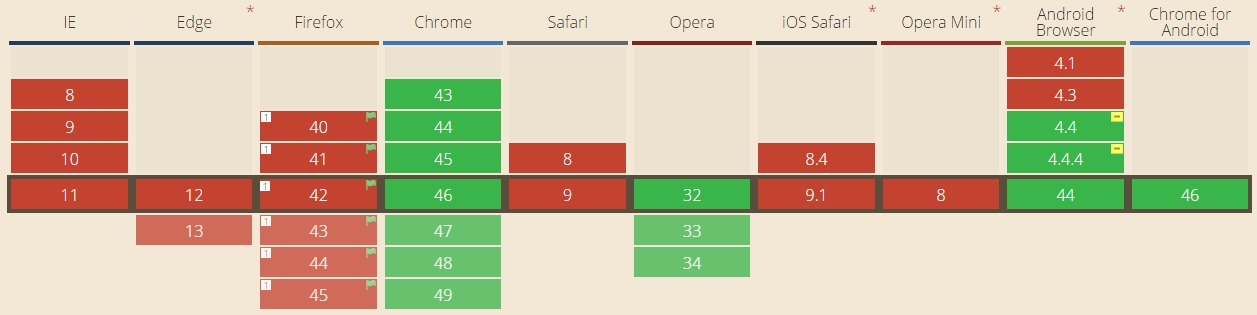
\includegraphics{images/2-shadow-dom-browserunterstuetzung.jpg}
\caption{Bild: Shadow DOM Browserunterstützung}
\end{figure}

{[}Can I Use 2015{]}

\subsection{Quellen}\label{quellen}

\begin{itemize}
\tightlist
\item
  {[}Developing Web Components 2015{]} Jarrod Overson \& Jason Strimpel,
  Developing Web Components, O'Reilly 2015, S.109-126
\item
  {[}Rob Dodson 2014{]} Rob Dodson, Shadow DOM CSS Cheat Sheet, 2014,
  http://robdodson.me/shadow-dom-css-cheat-sheet/
\item
  {[}Can I Use 2015{]} Can I Use,
  http://caniuse.com/\#search=shadow\%20dom
\item
  {[}Peter Kröner 2014{]} Peter Kröner, Das Web der Zukunft, 2014,
  http://webkrauts.de/artikel/2014/das-web-der-zukunft
\item
  {[}Colin Ihrig 2012{]} Colin Ihrig, The Basics of the Shadow DOM,
  2012, http://www.sitepoint.com/the-basics-of-the-shadow-dom/
\item
  {[}Dominic Cooney 2013{]} Dominic Cooney, Shadow DOM 101, 2013,
  http://www.html5rocks.com/en/tutorials/webcomponents/shadowdom/
\item
  {[}Eric Bidelman 2014{]} Eric Bidelman, Shadow DOM 201, 2014,
  http://www.html5rocks.com/en/tutorials/webcomponents/shadowdom-201//
\item
  {[}Eric Bidelman 2013{]} Eric Bidelman, Shadow DOM 301, 2013,
  http://www.html5rocks.com/en/tutorials/webcomponents/shadowdom-301/
\end{itemize}
